\chapter{Analiza Comparativă al metodelor de segmentare semantică a imaginilor și de detecție a obiectelor}
\label{cap:contributii}
În acest capitol se face prezentarea contribuțiilor autorului: un studiu comparativ a metodelor existente de detecția obiectelor și segmentarea semantică a imaginilor bazate pe rețele neuronale convoluționale.\newline
Se vor analiza în detaliu algoritmii care au la bază inteligență artificială deorece performanța acestora în domeniul prelucrării imaginilor depășește semnificativ orice altă metodă (algoritmi de nivel mai jos, cum ar fi algoritmii de thresholding) datorită faptului că rețelele neuronale nu sunt influențate de zgomotul din imagini, dar și pentru că sunt capabile de a produce rezultate în timp real \cite{cat_amz}.


\section{Categorii de algoritmi de segmentarea imaginilor}
Segmentarea imaginilor este unul dintre cele mai importante procese în domeniul viziunii artificiale moderne. Segmentarea imaginilor înseamnă etichetarea fiecărui pixel, ca aparținând unui obiect din imagine. Segmentele rezultate corespund unităților structurale (obiecte) din scenă. Segmentarea imaginilor este o problemă dificilă, pentru că nu există un model matematic care ar putea descrie bine procesul \cite{cat_amz}.\newline
Există un număr mare de algoritmi propuse în literatură, care vor fi prezentate în acest capitol. Favorizarea unei metode depinde numai de situație și de tipul de imagine care trebuie segmentat. Nu există nicio metodă universală, care produce rezultate bune pe fiecare tip de imagine. Chiar și alegerea metodei corespunzătoare pentru un tip de imagine este o problemă dificilă. Metode dezvoltate pentru un tip de imagine pot produce rezultate proaste pe alt tip de imagine.\newline
Technicile de segmentare pot fi plasate în trei clase mai mari:
\begin{itemize}
	\item algoritmi clasici bazate pe matematică sau metode statistice
	\item technici bazate pe inteligență artificială
	\item alte technici care fie sunt metode hibride, fie nu moștenesc din nicio categorie
\end{itemize}

Algoritmii clasici includ detecția marginilor obiectelor(\textit{edge/boundary detection)}, methode de thresholding (\textit{characteristic histogram thresholding)}, extragerea regiunilor (\textit{region extraction/region growing)} și abordări semantice și sintactice.\newline
Metodele de segmentare din domeniul inteligenței artificiale sunt de regulă metode care folosesc rețele neuronale.\newline

\subsection{Technici Bazate pe Rețele Neuronale Artificiale}
Începând cu anii 1990, rețelele neuronale au apărut și în domeniul prelucrării imaginilor și a viziunii artificiale. Având capabilități dorite (e.g. sunt insensibile la zgomotul din imagini, pot funcționa în timp real) au devenit foarte populare. Bineînțeles, diferite rețele neuronale au fost aplicate cu diferite nivele de succes; rețelele feed-forward back-propagation s-au dovedit a fi cele mai efective.\newline
Rețelele neuronale capabile de segmentare semantică pot fi împărțite în două categorii: rețele supravegheate și rețele nesupravegheate. Rețelele supravegheate au nevoie de set de antrenare etichetată, adică imagini pe care regiunile de interes sunt notate, având la îndemână și tipul obiectelor din zonele respective. Metodele nesupravegheate (numite și \textit{clustering processes}) sunt semi- sau total automate.

\subsubsection{Rețele supravegheate}
Rețelele neuronale care sunt antrenare cu învățare supravegheată au nevoie de un operator uman pentru a alege imaginile de antrenare și pentru a le segmenta în \textit{k} regiuni, fiecare fiind etichetat (cu tipul obiectului în regiune). Architectura propusă este antrenată folosind imaginile etichetate ca set de antrenare. După antrenare, rețeaua neuronală va fi capabilă de a segmenta imagini similare, asignând etichete pentru regiuni folosind cunoștințele acumulate la faza de antrenare.

\subsection{Algoritmi de Detectarea și Localizarea Obiectelor}
Este o confuzie generală între clasificarea imaginilor și detecția obiectelor din scene. Clasificarea imaginilor (\textit{image classification}) constă în obținerea unei predicții la ieșirea unui sistem referitor la tipul de obiect care era plasat în imaginea de intrare. Pe de altă parte, dacă vrem să identificăm locația obiectelor într-o imagine, și de exemplu să le numărăm numărul instanțelor unui obiect, putem folosi algoritmi de detecția obiectelor (\textit{object detection and localization}).\newline
%IoU Intersect over Union
\begin{figure}[h!]
    	\centering
	\captionsetup{justification=centering, margin=2cm}
	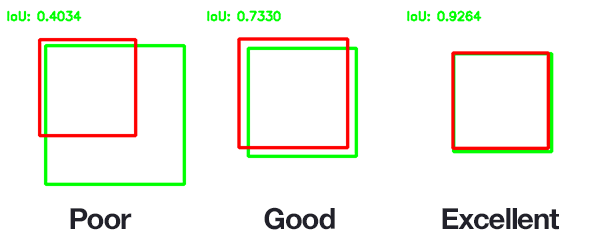
\includegraphics[width=0.5\textwidth]{figures/iou.png}
	\caption{Detecția obiectelor \cite{class_detect_segment}}
	\label{fig:class_detect_segment}
\end{figure}

\subsubsection{IoU - Intersect over Union}
Eficiența unui algoritm de localizare se măsoară folosind un algoritm de \textit{Intersect over Union}. Intersect over Union este o metodă pentru a evalua cât de aproape sunt predicțiile unui algoritm de detecția obiectelor de adevăr. \newline
Când vrem să măsurăm performanța rețelei antrenate, la stratul de intrare dăm imagini conținând obiecte care pot fi recunoscute și localizate de rețea, acesta specificând la stratul de ieșire predicția coordonatelor bounding-boxului fiecărui obiect. Aceste coordonate se compară cu cele reale, și se calculează Intersect over Union între dreptunghiurile definite de coordonatele specificate de rețea și dreptunghiurile reale (imaginile fiind etichetate avem la îndemână dreptunghiurile care conțin cu adevărat obiectele din imagini).
%object detection and localization
\begin{figure}[h!]
    	\centering
	\captionsetup{justification=centering, margin=2cm}
	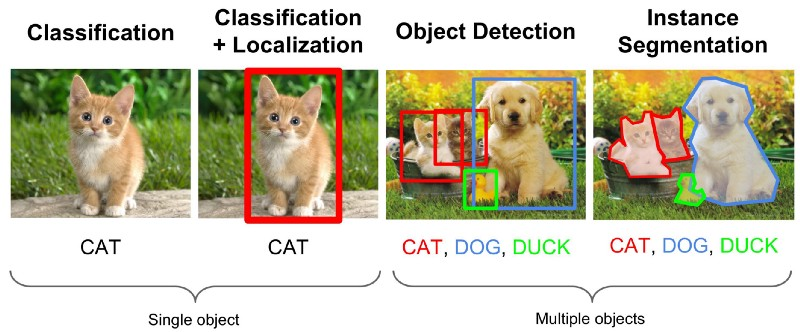
\includegraphics[width=0.9\textwidth]{figures/class_detect_segment.jpeg}
	\caption{Detecția obiectelor \cite{class_detect_segment}}
	\label{fig:class_detect_segment}
\end{figure}

Cinci abordări pentru detecția și localizarea obiectelor vor fi analizate și comparate:
\begin{itemize}
	\item RCNN
	\item Fast RCNN
	\item Faster RCNN
	\item Yolo
	\item SSD
\end{itemize}

\subsubsection{RCNN}
Când se face detectarea obiectelor o problemă cu care ne întâlnim inevitabil este faptul că în majoritatea cazurilor nu o să fie numai un bounding box pentru o scenă pentru că imaginea respectivă poate să conțină numeroase obiecte de interes și nu putem să știm dinainte câte. Din acest motiv nu putem să folosim o rețea neuronală standard extinsă cu un strat fully connected.\newline
RCNN (Regions + CNN) este o metodă care se bazează pe o metodă externă de propunere de regiuni care găsește regiunile de interes, și le găsește repede. Algoritmul extern de propunere de regiuni se numește \textit{selective search}.\newline
Chiar și accelerând pasul de generare de regiuni de interes, problema cu RCNN este că nu este destul de rapid.\newline
Cu ajutorul selective search se generează 2000 de regiuni cu potențial mare de a conține vreun obiect de interes. Regiunile generate de selective search sunt numite propuneri de regiuni (\textit{region proposals}). Aceste propuneri de regiuni sunt introduse într-o rețea convoluțională care produce un vector de trăsături. Astfel rețeaua convoluțională funcționează ca un extractor de trăsături, iar stratul de ieșire conține trăsăturile extrase care sunt introduse într-un support vector machine pentru a clasifica prezența unui obiect în propunerea de regiune.\newline
RCNN are și câteva dezavantaje:
\begin{itemize}
	\item chiar și cu accelerarea pasului de propunere de regiuni timpul de antrenare a rețelei este lung, pentru că pentru fiecare imagine este nevoie de clasificarea a 2000 de propuneri de regiuni
	\item nu poate funcționa în timp real, pentru că detectarea obiectelor durează 47 de secunde în medie pentru imagine
	\item algoritmul selective search nu poate fi îmbunătățit, nici nu poate să învețe. Asta poate duce la generarea neadecvată a propunerilor de regiuni.
\end{itemize}

\subsubsection{Fast RCNN}
Autorii articolului de RCNN au rezolvat câteva din problemele modelului RCNN pentru a construi un algoritm mai rapid pentru detectarea obiectelor. Acest algoritm îmbunătăți se numește Fast RCNN și este similar cu RCNN. Însă în loc de introducerea propunerilor de regiuni într-un CNN, se introduc imaginile în CNN pentru a genera o hartă de trăsături extrase cu o rețea convoluțională. Din această mapă identificăm propunerile de regiuni și folosim un strat softmax pentru a produce predicții de clasificare pentru regiuni.\newline
Fast RCNN este mai rapid decât predecesorul lui pentru că nu trebuie să introducem 2000 propuneri de regiuni în rețeaua convoluțională de fiecare dată; în schimb operația de convoluție se face o dată per imagine, pentru a genera harta trăsăturilor convoluționale.

%RCNN vs Fast RCNN training and testing times
\begin{figure}[h!]
    	\centering
	\captionsetup{justification=centering, margin=2cm}
	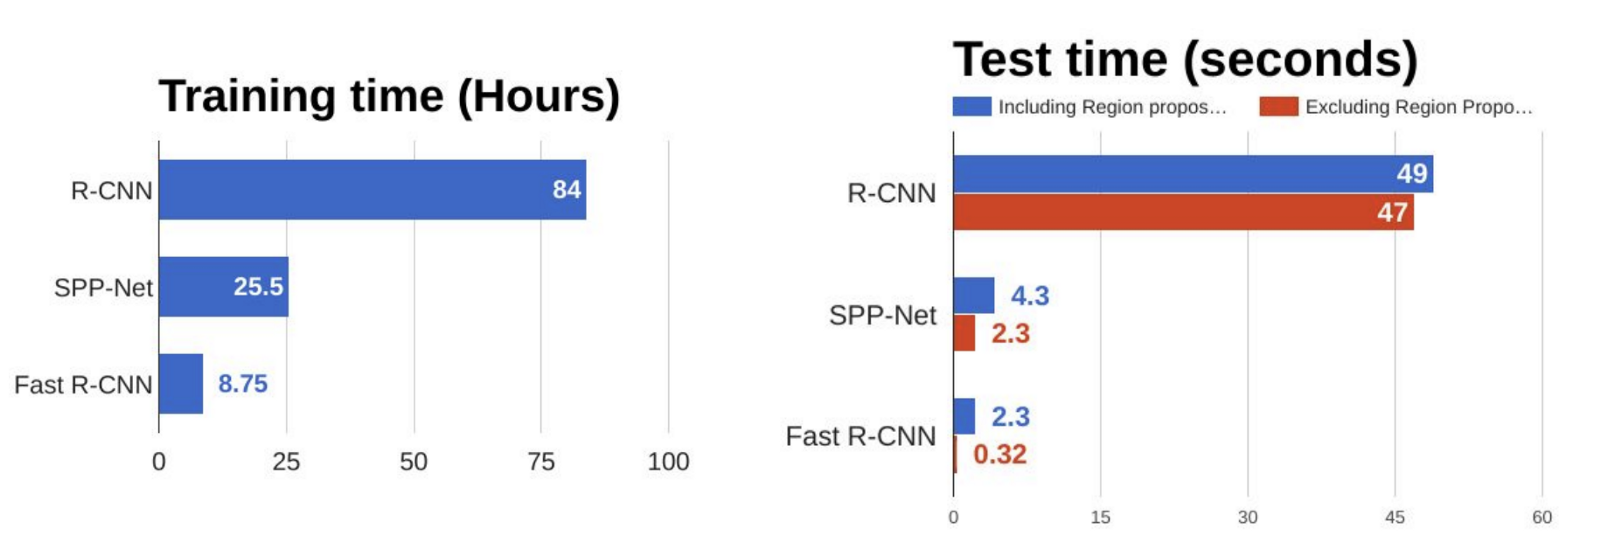
\includegraphics[width=0.9\textwidth]{figures/rcnn_vs_fast_rcnn_time.png}
	\caption{Diferența semnificativă dintre timpul de antrenare și testare între RCNN și Fast RCNN \cite{rcnn_vs_fast_rcnn}}
	\label{fig:class_detect_segment}
\end{figure}
Din acest grafic putem vedea că diferența dintre vitezele a rețelelor este semnificativă. Când ne uităm la performanța rețelei Fast RCNN observăm că performanța lui este mult mai bună fără folosirea metodei de propunere de regiuni. Deci algoritmul de propunere de regiuni este un bottleneck pentru Fast RCNN, afectând semnificativ performanța.

\subsubsection{Faster RCNN}
Ambii algoritmi de mai sus (RCNN și Fast RCNN) folosesc algoritmul selective search pentru a găsi propuneri de regiuni - regiuni cu potențial mare de a conține vreun obiect de interes. Acest algoritm este unul lent, consumă mult timp deci afectează performanța rețelei.\newline
Faster RCNN este similar cu Fast RCNN privind că și aici din imaginea introdusă se generează o hartă de trăsături convoluționale. În schimb aici nu se folosește selective search pentru a găsi regiunile de interes în harta de trăsături; în loc de acesta, o rețea separată este antrenată pentru a găsi predicții pentru coordonaterle regiunilor de interes. Regiunile previzionate sunt remodelate cu un strat RoI pooling și rezultatul este clasificat.

%RCNN vs Fast RCNN vs Faster RCNN testing time
\begin{figure}[h!]
    	\centering
	\captionsetup{justification=centering, margin=2cm}
	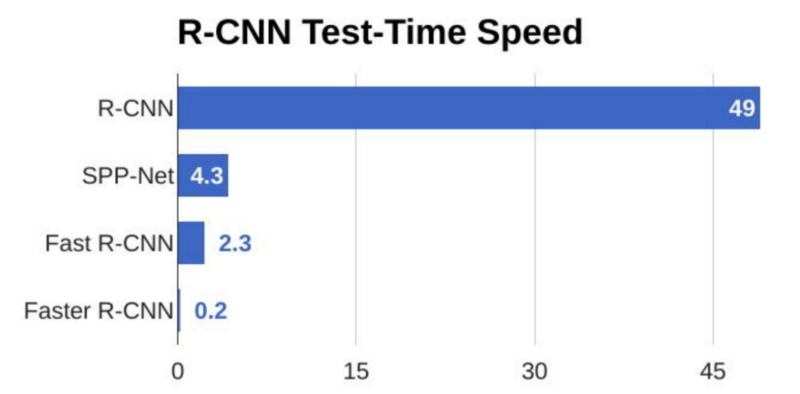
\includegraphics[width=0.8\textwidth]{figures/faster_rcnn_speed.png}
	\caption{Diferența dintre timpul de testare între  Fast RCNN și  Faster RCNN \cite{rcnn_vs_fast_rcnn}}
	\label{fig:class_detect_segment}
\end{figure}
Se vede că Faster RCNN este mult mai rapid decât predecesorii săi. Deja se poate folosi și pentru detectare de obiecte în timp real.\newline
Rețelele detaliate până aici au o trăsătură în comun: au o parte a rețelei dedicată pentru propunerea de regiuni, urmată de un clasificator performant. Aceste metode sunt capabile de o precizie ridicată, dar au dezavantajul că funcționează foarte lent (low frame-rate), însemnând că nu pot folosite în dispozitive embedded.\newline
O altă modalitate de a face detectare de obiecte este combinarea celor două pași (propuneri de regiuni și clasificare) într-o singură rețea. Acest scop poate fi atins cu o rețea care are un set predefinit de regiuni pentru găsirea obiectelor.\newline
O metodă pentru a refolosi rezultatul calculelor deja făcute la pasul de clasificare pentru localizare de obiecte este de a lua activările de la ultimul strat convoluțional. Aici încă avem informație spațială dar reprezentată într-o versiune mai mică decât în imaginea originală. De exemplu o imagine de 640x480x3 încărcată la stratul de intrare, pe ultimul strat convoluțional poate să producă ieșirea de dimensiunile 13x18x2048.\newline
Deci pe ultimul strat fiecare "pixel" reprezintă o zonă mai mare a imaginii de intrare, deci putem folosi aceste celule pentru a deduce poziția obiectelor.

%"pixels" from last layer correspond to larger areas on the original image
\begin{figure}[h!]
    	\centering
	\captionsetup{justification=centering, margin=2cm}
	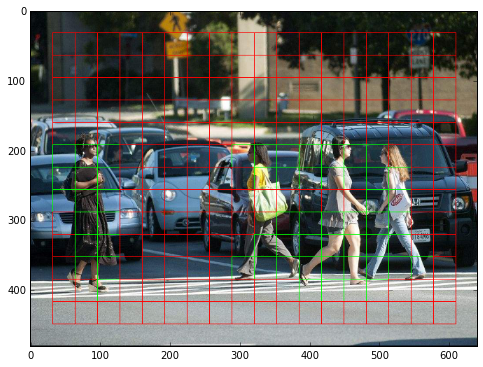
\includegraphics[width=0.8\textwidth]{figures/last_con_lay_to_inp_img.png}
	\caption{Diferența dintre timpul de testare între  Fast RCNN și  Faster RCNN \cite{rcnn_vs_fast_rcnn}}
	\label{fig:class_detect_segment}
\end{figure}

Un detaliu la care trebuie să fim atenți este că la folosirea fiecărui strat de pooling, pierdem o porțiune semnificativă de informație spațială.\newline
La acest pas putem folosi un strat convoluțional de 1x1 pentru a efectua o clasificare a fiecărei celule (e.g. pieton sau fundal), dar putem atașa încă un strat convoluțional sau fully-connected pentru a afla o predicție pentru cele 4 numere care descriu un bounding-box pentru obiectul conținut în celulă. Astfel primim clasificarea obiectului din regiune dar și locația sa.\newline
Este greșit să ne gândim ca și imaginea de intrare ar fi împărțită în celule înaintea începerii algoritmului. Ce se întâmplă de fapt este că fiecare strat reprezintă imaginea de intrare cu rezoluție mai mică, dar adâncime crescătoare. La antrenare facem a reconciliere între eticheta predefinită a imaginii și celulele virtuale (celulele pot să se suprapună).\newline
Familia detectoarelor de obiecte care folosesc această strategie:
\begin{itemize}
	\item SSD: folosește diferite matrice de activare (\textit{activation map}) pentru predicția claselor și a regiunilor
	\item YOLO: foloseste o singură matrice de activare pentru ambiele sarcini
	\item R-FCN (Region based Fully-Convolutional Neural Networks): funcționează mai rapid decât metodele (R-CNN, Fast R-CNN, etc) pentru că face puține calcule per celulă și este fully-conbolutional (conține numai straturi convoluționale).
\end{itemize}
Strategia acestor metode:
\begin{enumerate}
	\item se antrenează un CN cu regresiune (pentru bounding box) și clasificare (cu loss function)
	\item de obicei funcțiile de eroare sunt mai complexe pentru că trebuie să se descurce cu mai multe obiective (clasificare, regresiune, verificarea existenței unui obiect, etc.)
	\item culegerea activărilor de la un strat particular pentru a fi capabil de clasificare și localizare cu un strat FC sau un alt strat convoluțional
	 \item la pasul de prediction se folosesc algoritmi ca și \textit{non-maxima suppression} pentru a filtra multiple regiuni în jurul aceluiași obiect
	\item la stagiul de antrenare se folosesc algoritmi precum IoU (\textit{Intersect over Union}) pentru a afla corectitudinea localizării obiectului.
\end{enumerate}


\subsubsection{YOLO - You Only Look Once}
Până aici fiecare algoritm folosește regini pentru a localiza obiectele de interes în imagine. În loc să se uită la imaginea întreagă, rețeaua încearcă să găsească obiecte în părți care au potențial mare de a conține vreun obiect de interes.\newline
YOLO sau You Only Look Once este un algoritm de detectare de obiecte foarte diferit de algoritmii pe care le-am văzut până acum, fiindcă o singură rețea convoluțională este folosit atât pentru predicția bounding boxurilor cât și pentru clasificarea obiectelor din acestea.\newline
Acest detector are o precizie un pic mai mică dar funcționează foarte rapid (este capabil de detectare în timp real).

%YOLO functioning #1
\begin{figure}[h!]
    	\centering
	\captionsetup{justification=centering, margin=2cm}
	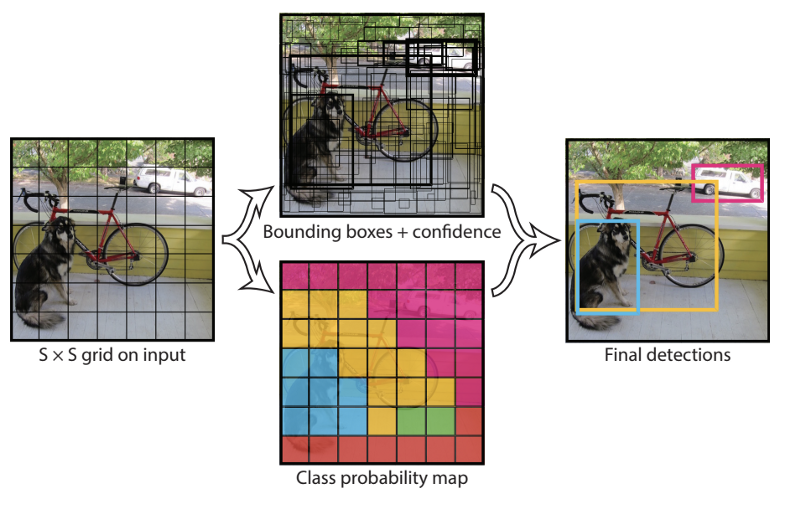
\includegraphics[width=0.8\textwidth]{figures/yolo1.png}
	\caption{YOLO \cite{rcnn_vs_fast_rcnn}}
	\label{fig:class_detect_segment}
\end{figure}

\paragraph{Ideea Principală}
Ideea din spatele acestui detector este că rulăm fiecare imagine printr-un model CNN și primim bounding boxes pentru obiecte într-un singur pas. Prima dată imaginea este redimensionată la rezoluția de 448x448, apoi încărcată în rețea. Ieșirea rețelei este filterată de un algoritm \textit{non-max suppression}.
Ieșirea modelului este un tensor batch de dimensiunile 7x7x30, și următorarele informații sunt codificate:
\begin{itemize}
	\item 2 definiții de bounding box: numere care identifică dreptungiul în care se află obiectul de interes (x, y, lățime, înălțime)
	\item 20 de probabilități de clase
\end{itemize}
Rețeaua este compuse folosind 9 straturi convoluționale, iar după ultimul strat de max-pool, din imaginea originală de 448x448 obținem o imagine de 7x7.\newline
Această ieșire de 7x7 poate fi considerată ca un grid de 7x7 reprezentând imaginea originală, unde fiecare celulă are 2 definiții de bounding box și 20 de probabilități de clase (celulele având o probabilitate de să aparțină unei clase din cele 20). Putem observa că această informație ne ajută și la detectarea clasei de obiect în care aparține entitatea din celulele respective.

%YOLO grid with possibilities
\begin{figure}[h!]
    	\centering
	\captionsetup{justification=centering, margin=2cm}
	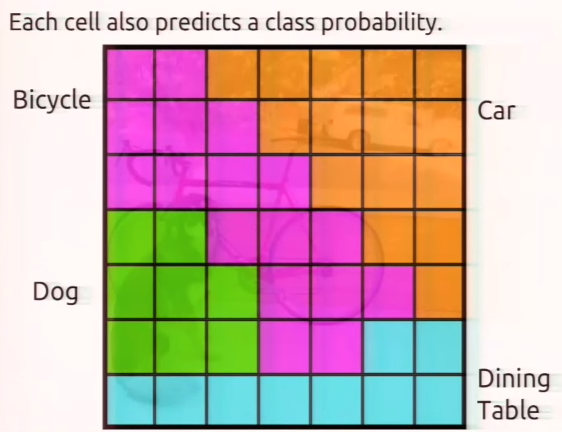
\includegraphics[width=0.7\textwidth]{figures/yolo_cell_class.png}
	\caption{YOLO \cite{rcnn_vs_fast_rcnn}}
	\label{fig:class_detect_segment}
\end{figure}

În ultimul pas folosind \textit{thresholding} și \textit{non-maxima suppression} putem filtra regiunile care nu sunt detectări valide.

\subsubsection{Multibox Single Shot Detector (SSD)}	
Detectorul SSD diferă de alte detectoare single-shot prin folosirea mai multor straturi care asigură o acuratețe mai bună în cazul obiectelor de mărimi diferente (cum straturile devin mai "adânci", ei sunt capabile de a observa obiecte mai mari).\newline
De obicei primul pas dintr-un single shot detector este un VGG pe un Resnet pre-antrenat care este convertit într-o rețea complet convoluțională. După aceasta se atașează câteva straturi convoluționale adiționale, ceea ce ne ajută la tratarea obiectelor mai mari. Architectura SSD se poate folosi de fapt împreună cu orice model bazat pe o rețea adâncă.\newline
Un lucru important de observat este faptul că după ce imaginea este introdusă în rețeaua VGG, câteva straturi convoluționale sunt adăugate pentru a produce hărți de trăsături de dimensiunile 19x19, 10x10, 5x5, 3x3, 1x1. Acestea împreună cu matricea de trăsături de 38x38 produsă de rețeaua VGG sunt matricele de trăsături folosite pentru a estima bounding boxes pentru obiectele de interes.\newline
Câteva activări sunt luate de la rețea și pasate într-o sub-rețea specializată care funcționează ca un clasificator și localizator. În faza de predicție se folosește algoritmul non-maxima suppression pentru a filtra multiple bounding-boxuri per obiect care pot să apară.


\subsection{Algoritmi de Segmentare Semantică}
Acum urmează să studiem detaliat algoritmii de segmentare semantică a imaginilor (\textit{semantic segmentation)}. Segmentare semantică este procedura prin care fiecărui pixel dintr-o imagine îi asignăm o etichetă care precizează cărui obiect aparține. Astfel algoritmii de segmentare semantică produc un \textit{map} a tuturor obiectelor detectate din imagine. Pe paginile următoare vom vedea cum funcționează diferite algoritmi bazate pe rețele neuronale convoluționale.

\subsubsection{Rețele Complet Convoluționale pentru Segmentare Semantică}
O rețea comple convoluțională seamănă foarte mult cu o rețea convoluțională normală, singura diferență fiind faptul că și ultimul strat este schimbat de încă un strat convoluțional. Ideea este că se capturează contextul global a scenei (să știm ce avem pe imagine și totodată să primim estimări despre locația obiectelor de interes).

%image segmentation fully convolutional
\begin{figure}[h!]
    	\centering
	\captionsetup{justification=centering, margin=2cm}
	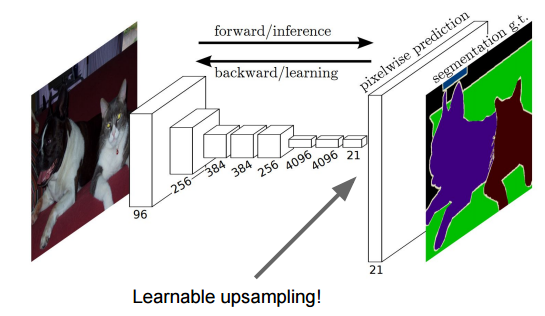
\includegraphics[width=0.7\textwidth]{figures/img_seg_ful_conv.png}
	\caption{Segmentare semantică \cite{rcnn_vs_fast_rcnn}}
	\label{fig:class_detect_segment}
\end{figure}

În 1990 rețelele neuronale convoluționale s-au dovedit folositoare pentru segmentarea semantică a imaginilor. Proprietățile lor dorite (eficiența nu se degradează în cazul imaginilor cu zgomot, capabile de a funcționa în timp real) au dus la aparența a multor modele și architecturi convoluționale. A varietate imensă de rețele convoluționale au fost aplicate pentru detectarea obiectelor și segmentarea semantică, cu mare succes. În această lucrare vom arunca o privire la rețele feed-forward back-propagation, Kohonen self organising maps, Hopfield neural networks, constraint satisfaction neural networks.\newline
Algoritmii de segmentare semantică bazate pe rețele neuronale pot fi împărțite în două categorii mari: algoritmi supravegheate și algoritmi nesupravegheate. Metodele supravegheate au nevoie de un set de antrenare etichetat (de oameni), adică un set de imagini segmentate de către experți humani. Pe de altă parte algoritmii nesupravegheați (sau procese de clustering) pot fi automate.

\subsubsection{Modele cu Învățare Supravegheată}













Titlul acestui capitol nu este unul impus și nici nu corespunde neapărat unui singur capitol. Titlul indică mai degrabă o parte (importantă și centrală, de altfel) a lucrării, în care se prezintă ceea ce s-a realizat efectiv: contribuțiile autorului. Organizarea acestei părți este dependentă și specifică fiecărei lucrări în parte și este stabilită de către fiecare autor după cum i se pare mai potrivit pentru tema lui. Ea poate cuprinde prezentarea unor concepte teoretice (unelte sau tehnici matematice folosite în lucrare, prezentarea sau introducerea unor concepte teoretice etc.), o analiză a diferitelor metode/algoritmi/tehnologii etc. luate în considerare sau dezvoltate de către autor, o prezentare a unui design (mai mult sau mai puțin detaliat) sau chiar detalii a unei eventuale implementări/prototip, dacă e cazul.

Trebuie remarcat însă faptul că această parte reprezintă contribuția personală a autorului, chiar dacă ea constă de exemplu doar dintr-o analiză comparativă a unor metode/algoritmi, și în nici un caz ea nu poate fi sinteza unor texte preluate din alte surse. Prin urmare, orice informații sunt prezentate aici, ele trebuie să corespundă cel puțin unei interpretări/analize critice personale a autorului, dacă nu chiar unor idei originale ale acestuia. 
